\documentclass[journal]{IEEEtran}
% \documentclass[journal,12pt,onecolumn,draftclsnofoot]{IEEEtran}

\usepackage[table]{xcolor}
\usepackage{adjustbox}
\usepackage{algorithm}
\usepackage{algpseudocode}
\usepackage{amsfonts}
\usepackage{amsmath}
\usepackage{amssymb}
\usepackage{amsthm}
\usepackage{bookmark}
\usepackage{booktabs}
\usepackage[makeroom]{cancel}
\usepackage[american]{circuitikz}
\usepackage{cite}
\usepackage{fixmath}
\usepackage[acronym]{glossaries-extra}
\usepackage{hyperref}
\usepackage{import}
\usepackage{mathtools}
\usepackage{microtype}
\usepackage[short]{optidef}
\usepackage{pgfplots}
\usepackage{ragged2e}
\usepackage[subtle]{savetrees}
\usepackage{siunitx}
\usepackage{stfloats}
\usepackage[caption=false,font=footnotesize,subrefformat=parens,labelformat=parens]{subfig}
\usepackage{tabularx}
\usepackage{tikz}
\usepackage{float}

% page limit hacks
% \usepackage{setspace}
% ! \usepackage[top=1cm, bottom=1cm, left=1cm, right=1cm]{geometry}
% \abovedisplayskip=1mm
% \belowdisplayskip=1mm
% \abovedisplayshortskip=1mm
% \belowdisplayshortskip=1mm
% \setlength{\jot}{0.1mm}
% \setlength{\floatsep}{1mm}
% \setlength{\textfloatsep}{1mm}
% \setlength{\intextsep}{1mm}
% \setlength{\skip\footins}{2mm}


% amsthm
\newtheorem{proposition}{Proposition}
\newtheorem{remark}{Remark}

% PGF/TikZ
\usetikzlibrary{arrows,calc,matrix,patterns,plotmarks,positioning,shapes}
\usetikzlibrary{decorations.pathmorphing,decorations.pathreplacing,decorations.shapes,shapes.geometric}
\usepgfplotslibrary{groupplots,patchplots}
\pgfplotsset{compat=newest}

% tabularx, ragged2e
\newcolumntype{L}{>{\RaggedRight}X}
\newcolumntype{C}{>{\centering\arraybackslash}X}
\renewcommand\tabularxcolumn[1]{m{#1}}

% algpseudocode
\makeatletter
\renewcommand{\fnum@algorithm}{\fname@algorithm{} \thealgorithm:}
\newcommand\setalgorithmcaptionfont[1]{%
	\let\my@floatc@ruled\floatc@ruled          % save \floatc@ruled
	\def\floatc@ruled{%
		\global\let\floatc@ruled\my@floatc@ruled % restore \floatc@ruled
		#1\floatc@ruled}}
\makeatother

\algrenewcommand{\algorithmicrequire}{\textbf{Input:}}
\algrenewcommand{\algorithmicensure}{\textbf{Output:}}
\algrenewcommand{\algorithmicwhile}{\textbf{While}}
\algrenewcommand{\algorithmicend}{\textbf{End}}
\algrenewcommand{\algorithmicrepeat}{\textbf{Repeat}}
\algrenewcommand{\algorithmicuntil}{\textbf{Until}}
\algrenewcommand{\algorithmicdo}{}

% glossaries-extra
\glsdisablehyper
\setabbreviationstyle[acronym]{long-short}
\newacronym{af}{AF}{Amplify-and-Forward}
\newacronym{ambc}{AmBC}{Ambient Backscatter Communication}
\newacronym{ap}{AP}{Access Point}
\newacronym{awgn}{AWGN}{Additive White Gaussian Noise}
\newacronym{bcd}{BCD}{Block Coordinate Descent}
\newacronym{bc}{BackCom}{Backscatter Communication}
\newacronym{bibo}{BIBO}{Binary-Input Binary-Output}
\newacronym{bpcu}{\si{bpcu}}{bits per channel use}
\newacronym{bpsphz}{\si{bps/Hz}}{bits per second per Hertz}
\newacronym{clt}{CLT}{Central Limit Theorem}
\newacronym{cw}{CW}{Continuous Waveform}
\newacronym{cp}{CP}{Canonical Polyadic}
\newacronym{cr}{CR}{Cognitive Radio}
\newacronym{cscg}{CSCG}{Circularly Symmetric Complex Gaussian}
\newacronym{csi}{CSI}{Channel State Information}
\newacronym{dc}{DC}{Direct Current}
\newacronym{df}{DF}{Decode-and-Forward}
\newacronym{dmc}{DMC}{Discrete Memoryless Channel}
\newacronym{dmtc}{DMTC}{Discrete Memoryless Thresholding Channel}
\newacronym{dmmac}{DMMAC}{Discrete Memoryless Multiple Access Channel}
\newacronym{dcmc}{DCMC}{Discrete-input Continuous-output Memoryless Channel}
\newacronym{dp}{DP}{Dynamic Programming}
\newacronym{fdma}{FDMA}{Frequency-Division Multiple Access}
\newacronym{iid}{i.i.d.}{independent and identically distributed}
\newacronym{ioe}{IoE}{Internet of Everything}
\newacronym{iot}{IoT}{Internet of Things}
\newacronym{kkt}{KKT}{Karush-Kuhn-Tucker}
\newacronym{m2m}{M2M}{Machine to Machine}
\newacronym{mac}{MAC}{Multiple Access Channel}
\newacronym{mc}{MC}{Multiplication Coding}
\newacronym{miso}{MISO}{Multiple-Input Single-Output}
\newacronym{mimo}{MIMO}{Multiple-Input Multiple-Output}
\newacronym{ml}{ML}{Maximum-Likelihood}
\newacronym{mrt}{MRT}{Maximum Ratio Transmission}
\newacronym{noma}{NOMA}{Non-Orthogonal Multiple Access}
\newacronym{ofdm}{OFDM}{Orthogonal Frequency-Division Multiplexing}
\newacronym{pdf}{PDF}{Probability Density Function}
\newacronym{pga}{PGA}{Projected Gradient Ascent}
\newacronym{psk}{PSK}{Phase Shift Keying}
\newacronym{qam}{QAM}{Quadrature Amplitude Modulation}
\newacronym{qos}{QoS}{Quality of Service}
\newacronym{rf}{RF}{Radio-Frequency}
\newacronym{rfid}{RFID}{Radio-Frequency Identification}
\newacronym{ris}{RIS}{Reconfigurable Intelligent Surface}
\newacronym{sc}{SC}{Superposition Coding}
\newacronym{sic}{SIC}{Successive Interference Cancellation}
\newacronym{simo}{SIMO}{Single-Input Multiple-Output}
\newacronym{sinr}{SINR}{Signal-to-Interference-plus-Noise Ratio}
\newacronym{smawk}{SMAWK}{Shor-Moran-Aggarwal-Wilber-Klawe}
\newacronym{snr}{SNR}{Signal-to-Noise Ratio}
\newacronym{sr}{SR}{Symbiotic Radio}
\newacronym{swipt}{SWIPT}{Simultaneous Wireless Information and Power Transfer}
\newacronym{tdma}{TDMA}{Time-Division Multiple Access}
\newacronym{ue}{UE}{user}
\newacronym{wit}{WIT}{Wireless Information Transfer}
\newacronym{wpcn}{WPCN}{Wireless Powered Communication Network}
\newacronym{wpt}{WPT}{Wireless Power Transfer}
\newacronym{mbc}{MBC}{Monostatic \glsentryshort{bc}}
\newacronym{bbc}{BBC}{Bistatic \glsentryshort{bc}}
\newacronym{bls}{BLS}{Backtracking Line Search}
\newacronym{mrc}{MRC}{Maximal Ratio Combining}
\newacronym{sdma}{SDMA}{Space-Division Multiple Access}
\newacronym{nlos}{NLoS}{Non-Line-of-Sight}
\newacronym{zf}{ZF}{Zero-Forcing}
\newacronym{mmse}{MMSE}{Minimum Mean-Square-Error}
\newacronym{fpga}{FPGA}{Field-Programmable Gate Array}
\newacronym{ber}{BER}{Bit Error Rate}

\begin{document}
\title{RIScatter: Unifying Backscatter Communication and Reconfigurable Intelligent Surface}
\author{
	\IEEEauthorblockN{
		Yang~Zhao,~\IEEEmembership{Member,~IEEE,}
		and~Bruno~Clerckx,~\IEEEmembership{Fellow,~IEEE}
	}
	\thanks{
		The authors are with the Department of Electrical and Electronic Engineering, Imperial College London, London SW7 2AZ, U.K. (e-mail: \{yang.zhao18, b.clerckx\}@imperial.ac.uk).
		B. Clerckx is also with Silicon Austria Labs (SAL), Graz A-8010, Austria.
	}
}
\maketitle

\begin{abstract}
	We propose RIScatter as a novel protocol that unifies \gls{bc} and \gls{ris} from a probabilistic perspective.
	In particular, batteryless scatter nodes powered by ambient transmission partially modulate their information and partially engineer the wireless channel.
	The key is to render the probability distribution of reflection states as a joint function of the information source, \gls{csi}, and relative priority of coexisting links.
\end{abstract}

\begin{IEEEkeywords}
	Active-passive coexisting network, input distribution design, \gls{sic}-free receiver.
\end{IEEEkeywords}

\glsresetall

\begin{section}{Introduction}
	\label{sc:introduction}
	\gls{ambc} has been recognized as a promising technology that allows low-power devices to charge and communicate wirelessly by recycling ambient radio waves \cite{Liu2013b}.
	The idea was extended to \gls{sr} where the legacy transmitter and passive node are cooperatively decoded by a co-located receiver \cite{Liang2020}.
	On the other hand, \gls{ris} is a passive signal reflector that customizes the wireless environment for signal enhancement, interference suppression, etc \cite{Wu2021b}.
	Those concepts essentially exploit the same physical mechanism of RF wave scattering/reflecting, but for different aims (backscatter modulation and passive beamforming).
\end{section}

\begin{section}{RIScatter}
	\label{sc:riscatter}
	For passive RIScatter nodes, each reflection state is simultaneously an information codeword and a passive beamforming codeword.
	The nodes randomize the reflection pattern over time while still guaranteeing the probability of occurrence of each state.
	This probability distribution is carefully designed to incorporate the backscatter information, \gls{csi}, and relative priority of both coexisting links.

	We also propose a low-complexity sequential decoding scheme that is readily applicable to legacy receivers.
	It semi-coherently decodes the weak backscatter signal using an energy detector, re-encodes for the exact reflection pattern, then coherently decodes the primary link.
	Therefore, backscatter detection can be viewed as part of channel training, and the impact of backscatter modulation can be modelled as dynamic passive beamforming.
	It only requires one additional energy comparison and re-encoding per backscatter symbol (instead of primary symbol), and can be tailored for arbitrary input distribution and spreading factor.

	In a single-user multi-node \gls{miso} RIScatter network, we characterize the achievable primary-(total-)backscatter rate region by optimizing the input distribution at RIScatter nodes, the active beamforming at the \gls{ap}, and the energy decision regions at the user under different \gls{qos}.
	Uniquely, our optimization problem takes into account the \gls{csi}, \gls{qos}, and backscatter constellation.
	This is the first proposal to reveal the importance of backscatter input distribution and decision region designs in active-passive coexisting networks.
\end{section}

\begin{section}{Results}
	\label{sc:simulation_results}
	\begin{figure}[H]
		\centering
		\subfloat[Input distribution: illustration]{
			\resizebox{0.7\columnwidth}{!}{
				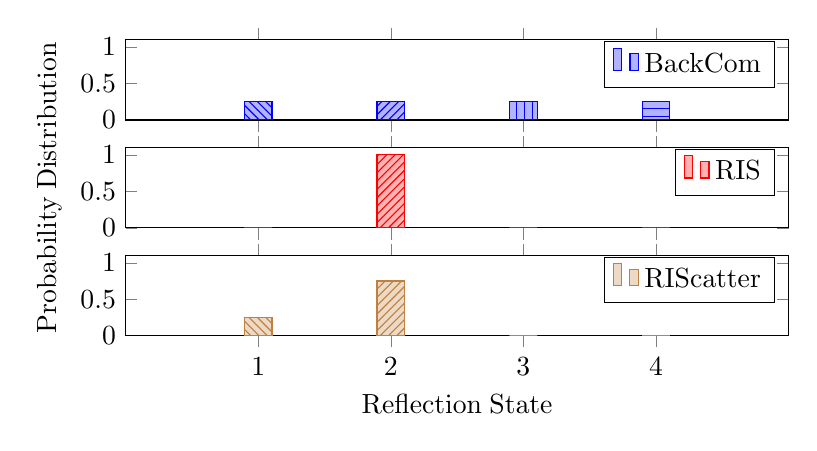
\begin{tikzpicture}
	\begin{groupplot}
		[group style={
					rows=3,
					group name=plots,
					x descriptions at=edge bottom,
					y descriptions at=edge left,
					vertical sep=10
				},
			ybar,
			xmin=0,
			xmax=4,
			xtick={1,2,3,4},
			ymin=0,
			ymax=1,
			xlabel={Reflection State},
			enlarge x limits={value=0.25,upper},
			enlarge y limits={value=0.1,upper},
			width=10cm,
			height=2.6cm,
			every axis plot/.append style={bar shift=0}
		]
		\nextgroupplot
		\addplot[blue,fill=blue!30!white] coordinates {(-1,-1)};
		\addplot[blue,fill=blue!30!white,postaction={pattern=north west lines},pattern color=.] coordinates {(1,0.25)};
		\addplot[blue,fill=blue!30!white,postaction={pattern=north east lines},pattern color=.] coordinates {(2,0.25)};
		\addplot[blue,fill=blue!30!white,postaction={pattern=vertical lines},pattern color=.] coordinates {(3,0.25)};
		\addplot[blue,fill=blue!30!white,postaction={pattern=horizontal lines},pattern color=.] coordinates {(4,0.25)};
		\legend{BackCom}
		\nextgroupplot[ylabel={Probability Distribution}]
		\addplot[red,fill=red!30!white] coordinates {(-1,-1)};
		\addplot[red,fill=red!30!white,postaction={pattern=north west lines},pattern color=.] coordinates {(1,0)};
		\addplot[red,fill=red!30!white,postaction={pattern=north east lines},pattern color=.] coordinates {(2,1)};
		\addplot[red,fill=red!30!white,postaction={pattern=vertical lines},pattern color=.] coordinates {(3,0)};
		\addplot[red,fill=red!30!white,postaction={pattern=horizontal lines},pattern color=.] coordinates {(4,0)};
		\legend{RIS}
		\nextgroupplot
		\addplot[brown,fill=brown!30!white] coordinates {(-1,-1)};
		\addplot[brown,fill=brown!30!white,postaction={pattern=north west lines},pattern color=.] coordinates {(1,0.25)};
		\addplot[brown,fill=brown!30!white,postaction={pattern=north east lines},pattern color=.] coordinates {(2,0.75)};
		\addplot[brown,fill=brown!30!white,postaction={pattern=vertical lines},pattern color=.] coordinates {(3,0)};
		\addplot[brown,fill=brown!30!white,postaction={pattern=horizontal lines},pattern color=.] coordinates {(4,0)};
		\legend{RIScatter}
	\end{groupplot}
\end{tikzpicture}

			}
			\label{fg:input_distribution_illustration}
		}
		\\
		\subfloat[Input distribution: simulation]{
			\resizebox{0.7\columnwidth}{!}{
				% This file was created by matlab2tikz.
%
%The latest updates can be retrieved from
%  http://www.mathworks.com/matlabcentral/fileexchange/22022-matlab2tikz-matlab2tikz
%where you can also make suggestions and rate matlab2tikz.
%
\definecolor{mycolor1}{rgb}{0.00000,0.44706,0.74118}%
\definecolor{mycolor2}{rgb}{0.85098,0.32549,0.09804}%
\definecolor{mycolor3}{rgb}{0.92941,0.69412,0.12549}%
\definecolor{mycolor4}{rgb}{0.49412,0.18431,0.55686}%
%
\begin{tikzpicture}

\begin{axis}[%
width=4.079in,
height=3.432in,
at={(0.684in,0.463in)},
scale only axis,
xmin=1,
xmax=4,
xtick={1, 2, 3, 4},
xlabel style={font=\color{white!15!black}},
xlabel={Reflection State},
ymin=0,
ymax=1,
ytick={  0, 0.2, 0.4, 0.6, 0.8,   1},
ylabel style={font=\color{white!15!black}},
ylabel={Probability Distribution},
axis background/.style={fill=white},
xmajorgrids,
ymajorgrids,
legend style={legend cell align=left, align=left, draw=white!15!black},
title style={font=\LARGE},
label style={font=\LARGE},
ticklabel style={font=\Large},
legend style={font=\Large}
]
\addplot [color=mycolor1, line width=2.0pt, mark=o, mark options={solid, mycolor1}]
  table[row sep=crcr]{%
1	5.58936301883394e-08\\
2	0.494967846198009\\
3	0.505032051077508\\
4	4.68308531955441e-08\\
};
\addlegendentry{$\rho =0$}

\addplot [color=mycolor2, dashed, line width=2.0pt, mark=+, mark options={solid, mycolor2}]
  table[row sep=crcr]{%
1	3.50493170830856e-09\\
2	0.586489834632108\\
3	0.413510159250847\\
4	2.6121135277758e-09\\
};
\addlegendentry{$\rho =0.1$}

\addplot [color=mycolor3, dotted, line width=2.0pt, mark=square, mark options={solid, mycolor3}]
  table[row sep=crcr]{%
1	1.54239700394178e-10\\
2	0.770075793479604\\
3	0.229924206275344\\
4	9.08124388871134e-11\\
};
\addlegendentry{$\rho =0.25$}

\addplot [color=mycolor4, dashdotted, line width=2.0pt, mark=x, mark options={solid, mycolor4}]
  table[row sep=crcr]{%
1	1.62167297049731e-12\\
2	0.999999185020827\\
3	8.14977502370884e-07\\
4	4.9209962545264e-14\\
};
\addlegendentry{$\rho =1$}

\end{axis}
\end{tikzpicture}%
			}
			\label{fg:input_distribution_simulation}
		}
		\caption{\gls{bc} and \gls{ris} can be viewed as extreme cases of RIScatter, where the input distribution boils down to uniform and degenerate. $\rho$ is the relative priority of the primary link.}
	\end{figure}
	At $\rho=0$ where the backscatter performance is prioritized, the optimal input distribution is \num{0} on two states and nearly uniform on the other two.
	This is inline with Shannon's observation that binary antipodal inputs is good enough for channel capacity at low \gls{snr} \cite{Shannon1948}.
	At $\rho=1$ where the primary link is prioritized, the optimal input distribution is $[0, 0, 1, 0]^\mathsf{T}$ since state 3 provides higher primary \gls{snr} than other states.
	That is, the reflection pattern becomes deterministic and the RIScatter node boils down to a static discrete \gls{ris} element.
	Increasing $\rho$ from \num{0} to \num{1} creates a smooth transition from backscatter modulation to passive beamforming, suggesting RIScatter unifies \gls{bc} and \gls{ris} from a probabilistic perspective.

	\begin{figure}[H]
		\centering
		\resizebox{0.7\columnwidth}{!}{
			% This file was created by matlab2tikz.
%
%The latest updates can be retrieved from
%  http://www.mathworks.com/matlabcentral/fileexchange/22022-matlab2tikz-matlab2tikz
%where you can also make suggestions and rate matlab2tikz.
%
\definecolor{mycolor1}{rgb}{0.30100,0.74500,0.93300}%
\definecolor{mycolor2}{rgb}{0.46600,0.67400,0.18800}%
\definecolor{mycolor3}{rgb}{0.49400,0.18400,0.55600}%
\definecolor{mycolor4}{rgb}{0.92900,0.69400,0.12500}%
\definecolor{mycolor5}{rgb}{0.85000,0.32500,0.09800}%
\definecolor{mycolor6}{rgb}{0.00000,0.44700,0.74100}%
%
\begin{tikzpicture}

\begin{axis}[%
width=4.079in,
height=1.587in,
at={(0.684in,0.361in)},
scale only axis,
xmin=0,
xmax=6.5227548374066,
xlabel style={font=\color{white!15!black}},
xlabel={Primary Rate [bits/s/Hz]},
ymin=0,
ymax=2,
ylabel style={font=\color{white!15!black}},
ylabel={Backscatter\\Rate [bits/BB]},
axis background/.style={fill=white},
xmajorgrids,
ymajorgrids,
legend style={at={(0.03,0.03)}, anchor=south west, legend cell align=left, align=left, draw=white!15!black},
align=center,
title style={font=\LARGE},
label style={font=\LARGE},
ticklabel style={font=\Large},
legend style={font=\Large},
reverse legend,
every axis plot/.append style={line width=2pt}
]
\addplot [color=mycolor1, line width=2.0pt, mark=triangle, mark options={solid, rotate=180, mycolor1}]
  table[row sep=crcr]{%
6.33724402501803	1.39764296268229\\
0	1.39764296268229\\
0	0\\
6.52275483678685	0\\
6.52275483678685	2.37312052924553e-08\\
6.38739454470992	1.3235811846854\\
6.35422040211439	1.38916612409166\\
6.34857862205488	1.39386686170527\\
6.3445353675389	1.39608085009443\\
6.34291602910554	1.3966977322109\\
6.34149846039129	1.39711118534274\\
6.34024731759122	1.39737797077851\\
6.3391350240222	1.3975379071887\\
6.33862394227692	1.39758701988787\\
6.33813974610465	1.39761939115801\\
6.33795313341839	1.39762818964178\\
6.33777036860279	1.39763482338317\\
6.3375913342378	1.3976394187338\\
6.33741590881855	1.39764209463684\\
6.33724402501803	1.39764296268229\\
};
\addlegendentry{RIScatter}

\addplot[only marks, mark=triangle, mark options={}, mark size=2.3570pt, draw=mycolor2] table[row sep=crcr]{%
x	y\\
6.5227548374066	0\\
};
\addlegendentry{RIS}

\addplot[only marks, mark=+, mark options={}, mark size=3.5355pt, draw=mycolor3] table[row sep=crcr]{%
x	y\\
6.34321982467796	2\\
};
\addlegendentry{SR}

\addplot[only marks, mark=x, mark options={}, mark size=3.5355pt, draw=mycolor4] table[row sep=crcr]{%
x	y\\
5.90778796357092	1.34857377961699\\
};
\addlegendentry{AmBC}

\addplot[only marks, mark=square, mark options={}, mark size=2.5000pt, draw=mycolor5] table[row sep=crcr]{%
x	y\\
0	1.99999999999997\\
};
\addlegendentry{BBC}

\addplot[only marks, mark=o, mark options={}, mark size=2.7386pt, draw=mycolor6] table[row sep=crcr]{%
x	y\\
6.34314881160129	0\\
};
\addlegendentry{Legacy}

\end{axis}
\end{tikzpicture}%
		}
		\caption{Achievable rate of different scattering applications. ``Legacy'' means active transmission without scatter nodes. ``BBC'' means bistatic \gls{bc}.}
		\label{fg:scatter_comparison}
	\end{figure}
	Fig.~\ref{fg:scatter_comparison} suggests RIScatter enables a flexible primary-backscatter tradeoff.
	In terms of maximum primary rate, RIScatter coincides with \gls{ris} and outperforms the others.
	On the other hand, the maximum backscatter rate is higher than that of \gls{ambc} thanks to adaptive active beamforming and input distribution design.
	To decode each backscatter symbol, \gls{sr} requires multiple re-encoding, precoding, subtraction and a time-domain \gls{mrc}, while RIScatter only requires one energy comparison and re-encoding.
	This allows RIScatter to achieve a higher backscatter throughput at a lower cost.
\end{section}

\begin{section}{Appendix}
	Full text is available at \url{https://arxiv.org/abs/2212.09121}.
	Source code will be released at \url{https://github.com/snowztail/riscatter}.
\end{section}

\bibliographystyle{IEEEtran}
\bibliography{../library.bib}
\end{document}
